\documentclass[12pt, reqno]{amsart}
\usepackage[margin = 0.5 in]{geometry}
\usepackage{multicol}
\usepackage{float}
\usepackage{fancyhdr}
\usepackage{graphicx}
\usepackage{hyperref}
\usepackage{fancyvrb}
\usepackage{physics}

\frenchspacing

\setlength{\abovecaptionskip}{5pt plus 3pt minus 3pt}

\hypersetup{colorlinks=true,allcolors=blue}
\pagestyle{fancy} \fancyhead{} \fancyfoot[C]{\normalsize\thepage}
\renewcommand{\headrulewidth}{0pt}
\begin{document}
\title{ME 5311 \quad Assignment 4 \quad Jacob Ivanov}

\maketitle
\begin{multicols}{2}
    \section{Model Diffusion Half-Life}
    The original PDE Diffusion model is defined as follows:
    \begin{equation}
        \begin{cases} \partial_t [u_k] = \alpha \cdot \partial_x^2 [u_k], \quad x \in [0, 2 \pi], \quad t \geq 0 \\
        u_k(t=0, x) = \sin(kx), \quad x \in [0, 2 \pi] \\
        u_k(t, x=0) = u_k(t, x = 2 \pi) = 0, \quad t \geq 0 \end{cases}
    \end{equation}
    By assuming Seperation of Variables:
    \begin{equation}
        u_k(t, x) = T(t) \cdot X(x)
    \end{equation}
    \begin{equation}
        T' X = \alpha T X''
    \end{equation}
    \begin{equation}
        \frac{T'}{T} = \alpha \frac{X''}{X} = c_1
    \end{equation}
    where $c_1$ is an arbitrary constant since $T'/T$ can only equal $X''/X$ if they are both the same constant.

    From which we can solve for $T$, $X$ independently:
    \begin{equation}
        T' - c_1 T = 0
    \end{equation}
    \begin{equation} \label{eq:6}
        X'' - \frac{\alpha}{c_1} X = 0
    \end{equation}
    if we assume an exponential form of $T = e^{\lambda t}$, it can be shown that $c_1 = \lambda$. As for $X$, if we assume a trigonometric form $X(x) = b_1 \cos(kx) + b_2 \sin(kx)$, find $X'$ and $X''$, plug into Eq. (6) and split by trigonometric term, it can be shown that $c_1 = - \alpha k^2$. As a result, our general solution (restricted to where $X(x)$ is trigonometric, rather than exponential) is as follows:
    \begin{equation}
        \begin{aligned}
        u_k(t, x) &= T(t) X(x) \\
        &= e^{-\alpha k^2 t} \left[ b_1 \cos(kx) + b_2 \sin(kx) \right]
        \end{aligned}
    \end{equation}

    If we apply our initial conditions (and indirectly our boundary conditions), it can be seen that $b_1 = 0$ and $b_2 = 1$. As a result, we are left with:
    \begin{equation}
        u_k(t, x) = e^{-\alpha k^2 t} \sin(kx)
    \end{equation}

    By defining a half-life time $t_{1/2}$ as follows, it can be directly found with some logarithm algebra.
    \begin{equation}
        u_k(t = t_{1/2}, x) = \frac{1}{2} u_k(t = 0, x)
    \end{equation}
    \begin{equation}
        t_{1/2}= \frac{\ln(2)}{\alpha k^2} \to t \propto \frac{1}{k^2}
    \end{equation}
    Therefore, the half-life decay time will be inversely proportional to the square of the wavenumber in the initial condition. For a linear combination of initial conditions, finer perturbations will decay quadratically faster than those on the large scale.

    \section{Model Advection}
    The advection phenomenon will be modelled as follows:
    \begin{equation}
        \begin{cases} \partial_t u(t, x) + \partial_x u(t, x) = 0\\
        u(t, x = 0) = \sin(8t), \quad t \in [0, 2] \\
        t \in [0, 2], \quad x \in [0, 1]
        \end{cases}
    \end{equation}
    Though the analytical solution can be found with the Method of Characteristics, we will instead solve it numerically with a Runge-Kutta 3rd Integration Method. To handle the right boundary, we will use a one sided finite difference. The solution at various times is shown below:
    \begin{figure}[H]
        \centering
        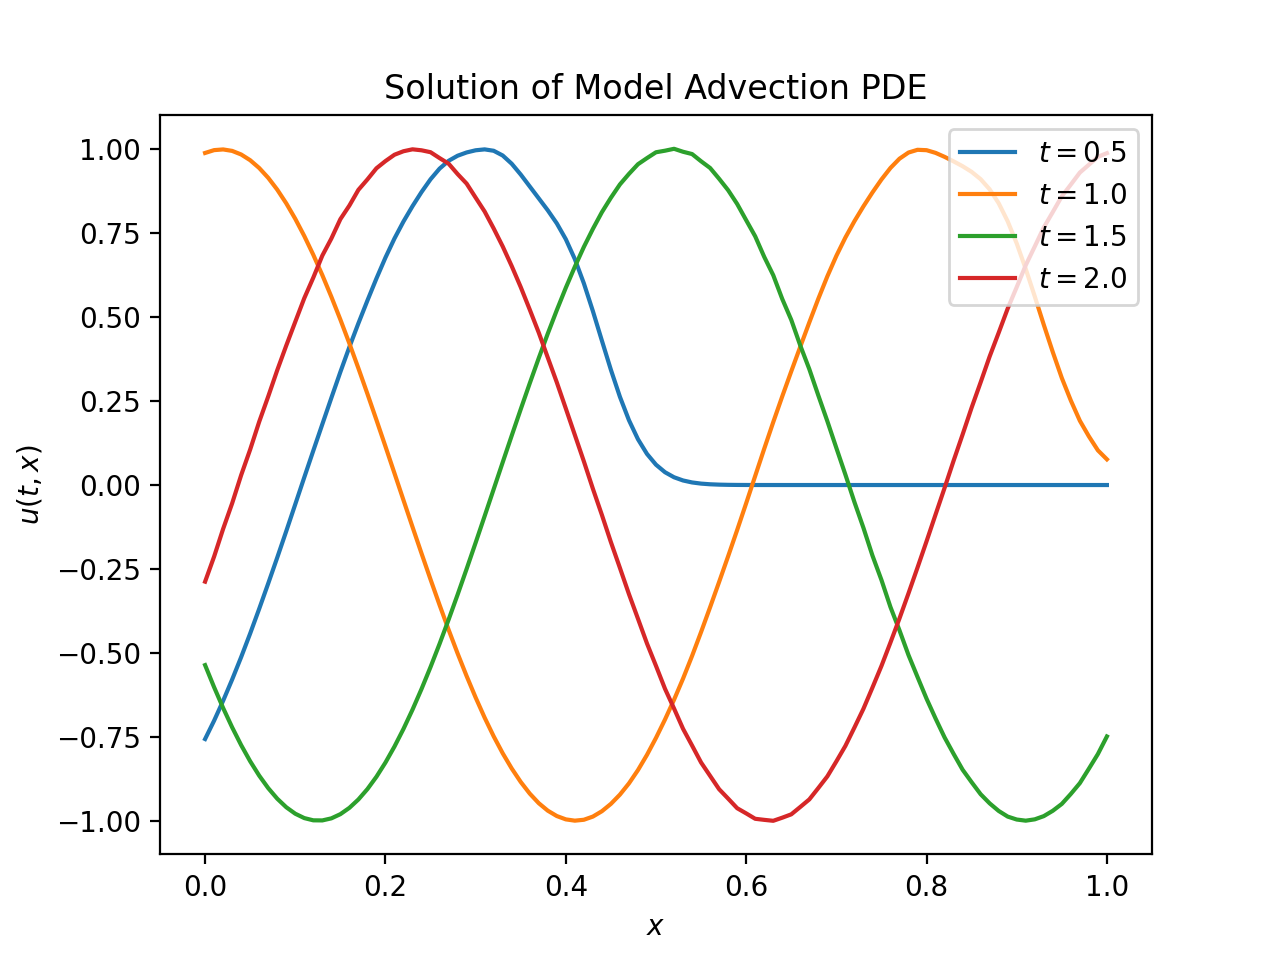
\includegraphics[width=1\linewidth]{Solution of Model Advection PDE.png}
    \end{figure}

\end{multicols}
\end{document}